\documentclass{bmstu}

\usepackage{mathtools}

\usepackage{physics}
\usepackage{pdfpages}
\usepackage{tabularx}
\usepackage{longtable}
\usepackage{xfrac}
\usepackage{amssymb}
\usepackage{dsfont}
\usepackage{upgreek}
\usepackage{color, colortbl}
\usepackage{listings}
\usepackage{ amssymb }
\usepackage{tikz}
\usetikzlibrary{decorations.markings}
\usetikzlibrary{calc} 

\begin{document}

   \section*{06/09}

\underline{Алгоритм метода конечных элементов:}
\begin{enumerate}
	\item Дискретизация;
	\item Аппроксимация кусочно-непрерывными функциями;
	\item Решение СЛАУ.
\end{enumerate}
	
	\begin{center}
		\textbf{Дискретизация области}
	\end{center}

\begin{enumerate}
		\item Разделение тела на конечные элементы;
		\item Нумерация ($N$ узлов, $N$ элементов).
\end{enumerate}

\begin{figure}[h] 
	\begin{center}
		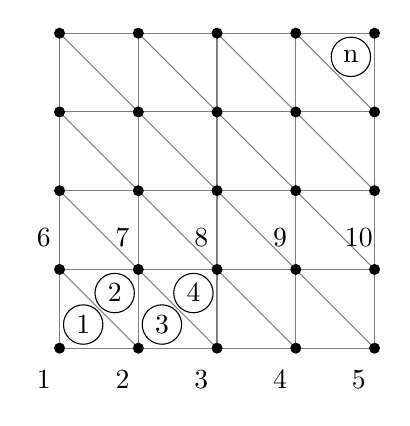
\begin{tikzpicture}
			\def\xmax{4}
			\def\ymax{4}
			
			\foreach \x in {0,1,...,\xmax} {
				\foreach \y in {0,1,...,\ymax} {
					\draw[gray] (\x, 0) -- (\x, \ymax);
					\draw[gray] (0, \y) -- (\xmax, \y);
				}
			}
			
			\foreach \x in {0,1,...,3} {
				\foreach \y in {0,1,...,3 } {
					\draw[gray] (\x, \y + 1) -- (\x + 1, \y);
				}
			}
			
			\foreach \x in {0,1,...,\xmax} {
				\foreach \y in {0,1,...,\ymax} {
					\fill (\x,\y) circle (2pt);
				}
			}
			
			\foreach \x in {1,2,...,5} {
				\node at (\x - 1.2, -0.4) {\x};
			}
			
			\foreach \x in {6,7,...,10} {
				\node at (\x - 6.2, 1.4) {\x};
			}
			
			\draw (0.3,0.3) circle (2.5mm); 
			\node at (0.3,0.3) {1}; 
			
			\draw (1.3,0.3) circle (2.5mm); 
			\node at (1.3,0.3) {3}; 
			
			\draw (0.7,0.7) circle (2.5mm); 
			\node at (0.7,0.7) {2}; 
			
			\draw (1.7,0.7) circle (2.5mm); 
			\node at (1.7,0.7) {4}; 
			
			\draw (3.7,3.7) circle (2.5mm); 
			\node at (3.7,3.7) {n}; 
			
		\end{tikzpicture}
	\end{center}
	\caption{Пример дискретизации области}
\end{figure}

\begin{figure}[h] 
	\begin{center}
		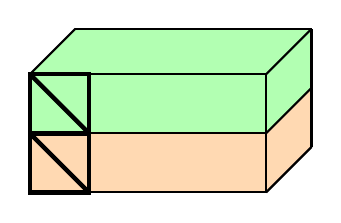
\begin{tikzpicture}[scale=1.5]
			\fill[orange!30] (0,0,1) -- (2,0,1) -- (2,0.5,1) -- (0,0.5,1) -- cycle;
			\fill[orange!30] (2,0,1) -- (2,0.5,1) -- (2,0.5,0) -- (2,0,0) -- cycle;
			
			\fill[green!30] (0,0.5,1) -- (2,0.5,1) -- (2,1,1) -- (0,1,1) -- cycle;
			\fill[green!30] (2,0.5,1) -- (2,1,1) -- (2,1,0) -- (2,0.5,0) -- cycle;
			\fill[green!30] (0,1,1) -- (2,1,1) -- (2,1,0) -- (0,1,0) -- cycle;
			
			
			\draw[thick] (0,0,1) -- (2,0,1) -- (2,1,1) -- (0,1,1) -- cycle; 
			
			\draw[thick] (2,0,0) -- (2,0,1); 
			\draw[thick] (2,1,0) -- (2,1,1); 
			\draw[thick] (0,1,0) -- (0,1,1); 
			\draw[thick] (2,0,0) -- (2,1,0); 
			\draw[thick] (0,1,0) -- (2,1,0); 
			
			\draw[thick] (0,0.5,1) -- (2,0.5,1); 
			\draw[thick] (2,0.5,0) -- (2,0.5,1);
			
			\draw[black, ultra thick] (0,0,1) rectangle (0.5,0.5,1);
			\draw[black, ultra thick] (0,0.5,1) rectangle (0.5,1,1);
			\draw[ultra thick] (0,0.5,1) -- (0.5,0,1);
			\draw[ultra thick] (0,1,1) -- (0.5,0.5,1);
			
			
		\end{tikzpicture}
	\end{center}
	\caption{Пример трехмерной области, состоящей из двух материалов}
\end{figure}

	\begin{figure}[H] 
	\begin{center}
		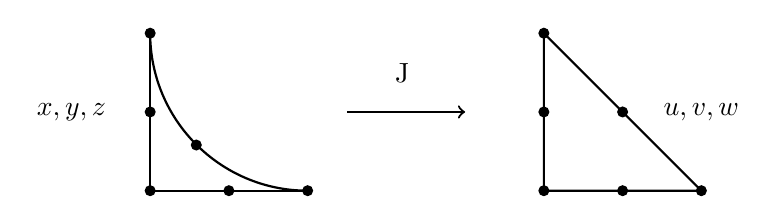
\begin{tikzpicture}
			
			\draw[thick] (0,0) arc[start angle=180, end angle=270, radius=2cm];
			\draw[thick] (2,-2) -- (0,-2);
			\draw[thick] (0,-2) -- (0,0);
			
			\draw[thick] (7,-2) -- (5,-2) -- (5,0)  -- cycle; 
			
			\draw[->, thick] (2.5,-1) -- (4,-1) ;
			\node at (3.2,-0.5) {J}; 
			
			\node at (-1,-1) {$x,y,z$};
			\node at (7,-1) {$u,v,w$};
			
			\fill (2,-2) circle (2pt);
			\fill (1,-2) circle (2pt);
			\fill (0,-2) circle (2pt);
			\fill (0,-1) circle (2pt);
			\fill (0,0) circle (2pt);
			\fill (0.58579, -1.42) circle (2pt);
			
			\fill (7,-2) circle (2pt);
			\fill (6,-2) circle (2pt);
			\fill (5,-2) circle (2pt);
			\fill (5,-1) circle (2pt);
			\fill (5,0) circle (2pt);
			\fill (6, -1) circle (2pt);
			
			
		\end{tikzpicture}
	\end{center}
	\caption{Приведение криволинейного элемента}
\end{figure}

\newpage
\underline{Замечания по разбиению:}
\begin{enumerate}
	\item Форма элемента должна быть близка к правильной;
	
\begin{figure}[h] 
	\begin{center}
		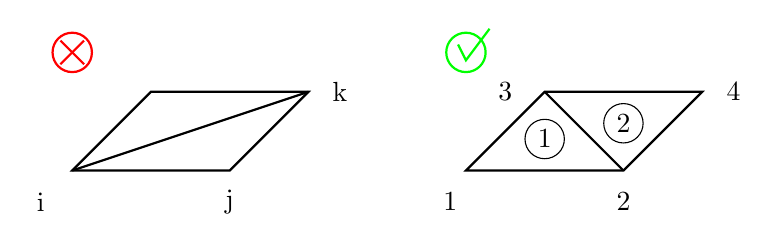
\begin{tikzpicture}
			
			\draw[thick] (0,0) -- (1,1) -- (3,1) -- (2,0)  -- cycle; 
			\draw[thick] (0,0) -- (3,1);
			
			\draw[thick] (5,0) -- (6,1) -- (8,1) -- (7,0)  -- cycle; 
			\draw[thick] (7,0) -- (6,1);
			
			\node at (-0.4,-0.4) {i};
			\node at (2,-0.4) {j};
			\node at (3.4,1) {k};
			
			\node at (4.8,-0.4) {1};
			\node at (7,-0.4) {2};
			\node at (5.5,1) {3};
			\node at (8.4,1) {4};
			
			\draw[red, thick] (0,1.5) circle (2.5mm);
			\draw[red, thick] (-0.15, 1.5-0.15) -- (0.15, 1.5+0.15);
			\draw[red, thick] (-0.15, 1.5+0.15) -- (0.15, 1.5-0.15);
			
			\draw[green, thick] (5,1.5) circle (2.5mm);
			\draw[green, thick] (4.9, 1.5+0.1) -- (5, 1.5-0.1) -- (5.3, 1.5+0.3);
			
			\draw (6,0.4) circle (2.5mm); 
			\node at (6,0.4) {1}; 
			
			\draw (7,0.6) circle (2.5mm); 
			\node at (7,0.6)  {2}; 
			
		\end{tikzpicture}
	\end{center}
	\caption{Пример плохой и хорошей дискретизации}
\end{figure}
	
	\item Все узлы конечного элемента должны совпадать.
	
	\begin{figure}[h] 
		\begin{center}
			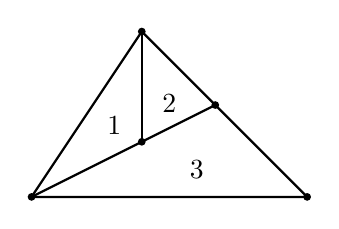
\begin{tikzpicture}[scale=0.7]
				
				\draw[thick] (0,0) -- (5,0) -- (2,3)  -- cycle; 
				\draw[thick] (0,0) -- (3.33333, 1.66667);
				\draw[thick] (2,3) -- (2,1);
				
				\fill (0,0) circle (2pt);
				\fill (5,0) circle (2pt);
				\fill (2,3) circle (2pt);
				\fill (3.33333, 1.66667) circle (2pt);
				\fill (2,1) circle (2pt);
				
				\node at (1.5,1.3) {1};
				\node at (2.5,1.7) {2};
				\node at (3,0.5) {3};
				
				
			\end{tikzpicture}
		\end{center}
		\caption{Пример плохой дискретизации}
	\end{figure}
	
\end{enumerate}

\underline{Замечание по нумерации узлов и конечных элементов:}

От нумерации узлов зависит ширина полосы ленты СЛАУ, поэтому узлы нужно нумеровать с короткой стороны для достижения наименьшей разницы между номерами узлов. Нумерация конечных элементов не важна, т.к. они привязаны к узлам.

\[
B=(R+1)\cdot Q
\]

где $B$ - ширина полосы ленты;

$R$ - максимальная по элементам величина наибольшей разности между узлами отдельного конечного элемента;

$Q$ - кол-во степенй свободы (число неизвестных).

\newpage
\underline{Нумерация треугольников против ЧС, начало с отдельных узлов.}
\begin{figure}[h] 
	\begin{center}
		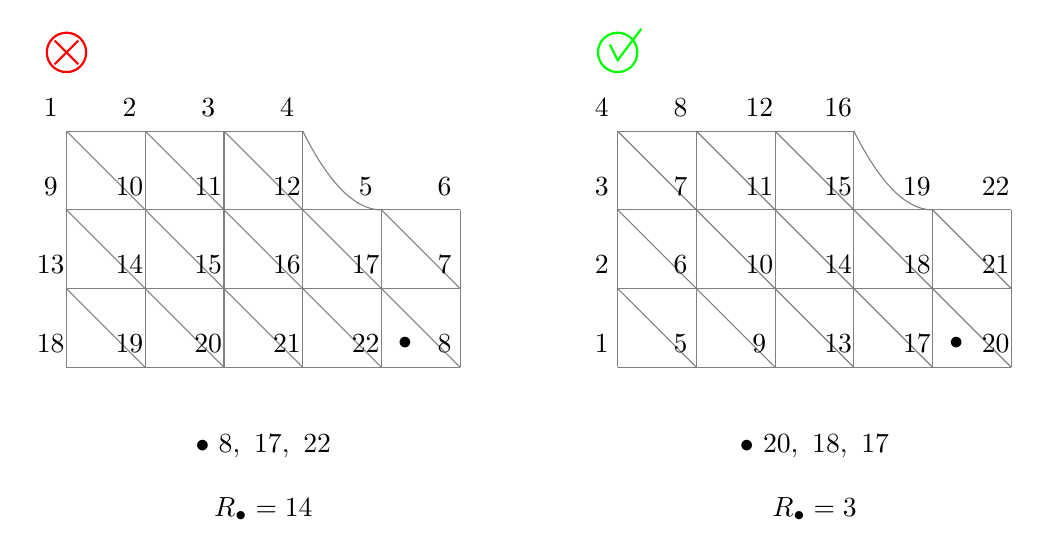
\begin{tikzpicture}[domain = -1:0] 
			\foreach \x in {0,1,...,3} {
				\foreach \y in {0,1,...,3} {
					\draw[gray] (\x, 0) -- (\x, 3);
					\draw[gray] (0, \y) -- (3, \y);
				}
			}
			
			\foreach \x in {0,1,...,2} {
				\foreach \y in {0,1,...,2 } {
					\draw[gray] (\x, \y + 1) -- (\x + 1, \y);
				}
			}
			
			\foreach \x in {0,1,...,2} {
				\foreach \y in {0,1,...,2} {
					\draw[gray] (\x+3, 0) -- (\x+3, 2);
					\draw[gray] (3, \y) -- (5, \y);
				}
			}
			
			\foreach \x in {0,1} {
				\foreach \y in {0,1} {
					\draw[gray] (\x+3, \y + 1) -- (\x + 4, \y);
				}
			}
			
			\draw[gray] plot (\x+4, \x * \x+2);
			
			\foreach \x in {1,2,...,4} {
				\node at (\x - 1.2, 3.3) {\x};
			}
			
			\foreach \x in {9,10,...,12} {
				\node at (\x - 9.2, 2.3) {\x};
			}
			
			\foreach \x in {13,14,...,17} {
				\node at (\x - 13.2, 1.3) {\x};
			}
			
			\foreach \x in {18,19,...,22} {
				\node at (\x - 18.2, 0.3) {\x};
			}
			
			\node at (3.8, 2.3) {5};
			
			\foreach \x in {6,7,...,8} {
				\node at (4.8, 8.3 - \x) {\x};
			}
			
			\node at (4.3, 0.3) {$\bullet$};
			\node at (2.5,-1) {$\bullet\ 8,\ 17,\ 22$};
			\node at (2.5,-1.8) {$R_\bullet = 14$};
			
			%second pic
			\foreach \x in {7,8,...,10} {
				\foreach \y in {0,1,...,3} {
					\draw[gray] (\x, 0) -- (\x, 3);
					\draw[gray] (7, \y) -- (10, \y);
				}
			}
			
			\foreach \x in {0,1,...,2} {
				\foreach \y in {0,1,...,2 } {
					\draw[gray] (\x+7, \y + 1) -- (\x + 8, \y);
				}
			}
			
			\foreach \x in {7,8,...,9} {
				\foreach \y in {0,1,...,2} {
					\draw[gray] (\x+3, 0) -- (\x+3, 2);
					\draw[gray] (10, \y) -- (12, \y);
				}
			}
			
			\foreach \x in {0,1} {
				\foreach \y in {0,1} {
					\draw[gray] (\x+10, \y + 1) -- (\x + 11, \y);
				}
			}
			
			\draw[gray] plot (\x+11, \x * \x+2);
			
			\foreach \x in {1,2,...,4} {
				\node at (6.8, -0.7+\x) {\x};
			}
			
			\foreach \x in {5,6,...,8} {
				\node at (7.8, -4.7+\x) {\x};
			}
			
			\foreach \x in {9,10,...,12} {
				\node at (8.8, -8.7+\x) {\x};
			}
			
			\foreach \x in {13,14,...,16} {
				\node at (9.8, -12.7+\x) {\x};
			}
			
			\foreach \x in {17,18,...,19} {
				\node at (10.8, -16.7+\x) {\x};
			}
			
			\foreach \x in {20,21,...,22} {
				\node at (11.8, -19.7+\x) {\x};
			}
			
			\node at (11.3, 0.3) {$\bullet$};
			\node at (9.5,-1) {$\bullet\ 20,\ 18,\ 17$};
			\node at (9.5,-1.8) {$R_\bullet = 3$};
			
			
			\draw[red, thick] (0,4) circle (2.5mm);
			\draw[red, thick] (-0.15, 4-0.15) -- (0.15, 4+0.15);
			\draw[red, thick] (-0.15, 4+0.15) -- (0.15, 4-0.15);
			
			\draw[green, thick] (7,4) circle (2.5mm);
			\draw[green, thick] (6.9, 4+0.1) -- (7, 4-0.1) -- (7.3, 4+0.3);
			
			
		\end{tikzpicture}
	\end{center}
	\caption{Пример правильной и неправильной нумерации узлов}
\end{figure}



Форма записи КЭ в файл(трехмерный случай):
\[
	\begin{rcases*}
		\begin{matrix}
			1 & x_1 & y_1 & z_1 \\
			2 & x_2 & y_2 & z_2 \\
			\cdots & \cdots & \cdots & \cdots\\
			n & x_n & y_n & z_n \\
		\end{matrix}
	\end{rcases*}
	\text{номера узлов и их координаты} 
\]

\[	
	\begin{rcases*}
		\begin{matrix}
			\textcircled{1} & 1 & 2 & 3 \\
			\textcircled{2} & 4 & 3 & 2 \\
			\cdots & \cdots & \cdots & \cdots\\
			\textcircled{n} & \cdots & \cdots & \cdots\\
		\end{matrix}
	\end{rcases*}
	\begin{matrix}
		\text{номера КЭ и номера узлов, из}  \\
		\text{которых они состоят}
	\end{matrix}	
\] 
\newpage
\indent \underline{Замечания о порядке узлов, составляющих КЭ:} 
\begin{enumerate}
	\item Обход узлов КЭ принято делать против часовой стрелки (для того, чтобы нормали были направлены в одну сторону); 
	\item Нумерацию желательно делать таким образом, чтобы соответствующие узлы попали в одно и то же место СЛАУ. 
\end{enumerate} 

\indent Пояснение к замечанию 2: \\
\indent Обратимся к Рисунку 4. Представим, что мы накладываем один КЭ на другой. Первый КЭ начнем нумеровать с узла №1 --- (1-2-3), тогда второй КЭ начнем обходить с узла №4 --- (4-3-2) и тд.

   \newpage
   	\section*{13/09}
	
	\begin{center}
	\textbf{Одномерные пружинные системы}
	\end{center}
	
	 \begin{figure}[h] 
	\begin{center}
	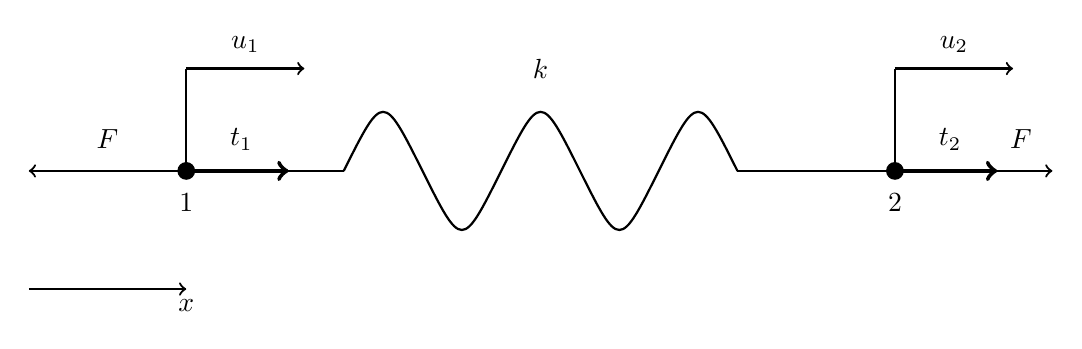
\begin{tikzpicture}
	\draw[thick] (-2, 0) -- (0, 0);
    \draw[thick] (0,0) 

        .. controls +(0.5,1) and +(-0.5,1) .. (1,0)
        .. controls +(0.5,-1) and +(-0.5,-1) .. (2,0)
        .. controls +(0.5,1) and +(-0.5,1) .. (3,0)
        .. controls +(0.5,-1) and +(-0.5,-1) .. (4,0)
        .. controls +(0.5,1) and +(-0.5,1) .. (5,0);
        
       	\node at (2.5, 1.3) {$k$};

    \draw[thick] (5,0);
    \draw[thick] (5, 0) -- (7, 0);
    
    \filldraw (-2, 0) circle (3pt);
     \node  at (-2,-0.4) {1};
    \filldraw (7, 0) circle (3pt);
     \node  at (7,-0.4) {2};
    
    \draw[->][ultra thick] (-2,0) -- (-0.7,0);
    \draw[->][ultra thick] (7,0) -- (8.3,0);
    \node at (-1.3, 0.4) {$t_1$};
    \node at (7.7, 0.4) {$t_2$};
    
    \draw[->][thick] (-2,0) -- (-4,0);
    \draw[->][thick] (7,0) -- (9,0);
     \node at (-3, 0.4) {$F$};
    \node at (8.6, 0.4) {$F$};
    
    \draw[thick] (-2,0) -- (-2,1.3);
    \draw[thick] (7,0) -- (7,1.3);
    \draw[->][thick] (-2,1.3) -- (-0.5,1.3);
    \draw[->][thick] (7,1.3) -- (8.5,1.3);
    \node at (-1.25, 1.6) {$u_1$};
    \node at (7.75, 1.6) {$u_2$};
    
     \draw[->][thick] (-4,-1.5) -- (-2,-1.5) node[below] {$x$};
	\end{tikzpicture}
	\end{center}
	 \caption{Одномерная пружинная система из одного элемента}
 \end{figure}

	
	\textbf{1.} \underline{Уравнение равновесия}
	
	где $k$ - коэффициент жесткости, $u_1, u_2$ - перемещения, $F$ - приложенная сила, $t_1, t_2$ - реакции. 
	
	Закон Гука:
	\[
	F= k\Delta = k(u_2-u_1)
	\]
	\[
	t_1+t_2=0 \rightarrow t_1=-t_2
	\]
	\[
	F=t_2=k(u_2-u_1)
	\]
	\[
	-F=t_1=-k(u_2-u_1)=k(u_1-u_2)
	\]
	\[
	\begin{bmatrix}
		k & - k \\ -k & k
	\end{bmatrix}
	\begin{bmatrix}
	u_1 \\ u_2
	\end{bmatrix} = \begin{bmatrix}
	t_1 \\ t_2
	\end{bmatrix}  \Leftrightarrow Kq=t
	\]
	
	где $q = \begin{bmatrix}
		u_1 \\ u_2
	\end{bmatrix},\ t = \begin{bmatrix}
	t_1 \\ t_2
	\end{bmatrix}, \ K =	\begin{bmatrix}
	k & - k \\ -k & k
	\end{bmatrix}$.\\

\textbf{2.} \underline{Вариационный метод}

\[
\text{П} = \text{П}_{in} - \text{П}_{ex},
\]

где $\text{П}$ - потенциальная энергия системы. 
\[
\text{П}_{in} = \int\limits_0^{\Delta} Fd\Delta = \int\limits_0^{\Delta}k\Delta d\Delta = \frac{k(u_2-u_1)^2}{2}=\frac{1}{2}q^{\text{Т}}Kq=\frac{1}{2}\begin{bmatrix}
		u_1 & u_2
	\end{bmatrix}\begin{bmatrix}
	k & - k \\ -k & k
	\end{bmatrix}
	\begin{bmatrix}
	u_1 \\ u_2
	\end{bmatrix}
\]
\[
\text{П}_{ex} =  t_1 u_1 +t_2 u_2 = q^{\text{Т}}t
\]
\[
\text{П} = \frac{1}{2}q^{\text{Т}}Kq-q^{\text{Т}}t\rightarrow min
\]

Условие стационарности потенциальной энергии
\[
\frac{\partial \text{П}}{\partial q}=0 \Leftrightarrow \frac{\partial \text{П}}{\partial u_1}=0, \ \frac{\partial \text{П}}{\partial u_2}=0
\]
\[
\text{П}=\frac{k}{2}(u_2-u_1)^2-t_1u_1-t_2u_2
\]
\[
\frac{\partial \text{П}}{\partial u_1}=k(u_2-u_1)(-1)-t_1=0 \Leftarrow k(u_1-u_2)= t_1
\]
\[
\frac{\partial \text{П}}{\partial u_2}=k(u_2-u_1)-t_2=0 \Leftarrow k(u_2-u_1)= t_2
\]
\[
\begin{bmatrix}
	k & - k \\ -k & k
\end{bmatrix}
\begin{bmatrix}
	u_1 \\ u_2
\end{bmatrix} = \begin{bmatrix}
	t_1 \\ t_2
\end{bmatrix} 
\]

\textbf{3.} \underline{Метод возможных перемещений}

Работа внутренних сил на возможных деформациях равна внешней работе возможных перемещений:
\[
A_{in}=A_{ex},
\]

где $A_{in}$ - работа внутренних сил на возможных деформациях, 

$A_{ex}$ - работа внешних сил на возможных перемещениях.
\[
A_{in}=F\delta\Delta = F(\delta u_2- \delta u_1)
\]
\[
A_{ex}= t_1\delta u_1 + t_2\delta u_2
\]
\[
F(\delta u_2- \delta u_1)=t_1\delta u_1 + t_2\delta u_2
\]
\[
\delta u_1, \delta u_2 :  \begin{cases}
	- F=t_1 \\ F=t_2
\end{cases}
\]

\newpage
\textbf{Методика составления глобальной системы для МКЭ}

 \begin{figure}[h]
\begin{center}
	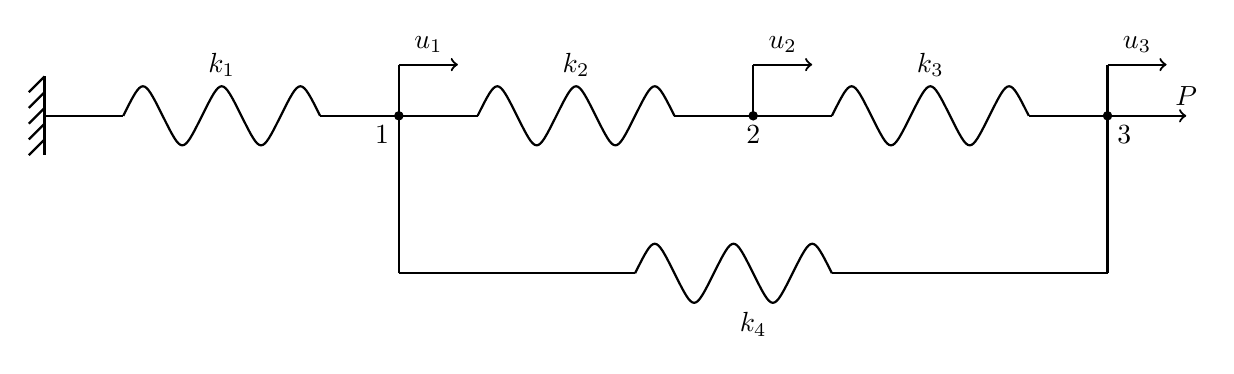
\begin{tikzpicture}[scale=0.5]
	%1 element
	\draw[thick] (-11, 1) -- (-11, -1);
	\draw[thick] (-11.4, 0.6) -- (-11, 1);
	\draw[thick] (-11.4, 0.2) -- (-11, 0.6);
	\draw[thick] (-11.4, -0.2) -- (-11, 0.2);
	\draw[thick] (-11.4, -0.6) -- (-11, -0.2);
	\draw[thick] (-11.4, -1) -- (-11, -0.6);
	
	\draw[thick] (-11, 0) -- (-9, 0);
    \draw[thick] (-9,0) 

        .. controls +(0.5,1) and +(-0.5,1) .. (-8,0)
        .. controls +(0.5,-1) and +(-0.5,-1) .. (-7,0)
        .. controls +(0.5,1) and +(-0.5,1) .. (-6,0)
        .. controls +(0.5,-1) and +(-0.5,-1) .. (-5,0)
        .. controls +(0.5,1) and +(-0.5,1) .. (-4,0);
        
       	\node at (-6.5, 1.3) {$k_1$};
	\draw[thick] (-4, 0);
    	\draw[thick] (-4, 0) -- (-2, 0);
	
	%2 element
	\draw[thick] (-2, 0) -- (0, 0);
    \draw[thick] (0,0) 

        .. controls +(0.5,1) and +(-0.5,1) .. (1,0)
        .. controls +(0.5,-1) and +(-0.5,-1) .. (2,0)
        .. controls +(0.5,1) and +(-0.5,1) .. (3,0)
        .. controls +(0.5,-1) and +(-0.5,-1) .. (4,0)
        .. controls +(0.5,1) and +(-0.5,1) .. (5,0);
        
       	\node at (2.5, 1.3) {$k_2$};

    \draw[thick] (5,0);
    \draw[thick] (5, 0) -- (7, 0);
    
    \filldraw (-2, 0) circle (3pt) node[below left] {1};
    \filldraw (7, 0) circle (3pt) node[below] {2};
    
    \draw[thick] (-2,0) -- (-2,1.3);
    \draw[thick] (7,0) -- (7,1.3);
    \draw[->][thick] (-2,1.3) -- (-0.5,1.3);
    \draw[->][thick] (7,1.3) -- (8.5,1.3);
    \node at (-1.25, 1.8) {$u_1$};
    \node at (7.75, 1.8) {$u_2$};
    
    %3 element
	\draw[thick] (7, 0) -- (9, 0);
    \draw[thick] (9,0) 

        .. controls +(0.5,1) and +(-0.5,1) .. (10,0)
        .. controls +(0.5,-1) and +(-0.5,-1) .. (11,0)
        .. controls +(0.5,1) and +(-0.5,1) .. (12,0)
        .. controls +(0.5,-1) and +(-0.5,-1) .. (13,0)
        .. controls +(0.5,1) and +(-0.5,1) .. (14,0);
        
       	\node at (11.5, 1.3) {$k_3$};
	\draw[thick] (14, 0);
    	\draw[thick][->] (14, 0) -- (18, 0) node[above] {$P$};
	
	\filldraw (16, 0) circle (3pt) node[below right] {3};
	
	 \draw[thick] (16,0) -- (16,1.3);
	 \draw[->][thick] (16,1.3) -- (17.5,1.3);
	 \node at (16.75, 1.8) {$u_3$};
	 
	 %4 element
	 \draw[thick] (-2, -4) -- (-2,0);
	\draw[thick] (-2, -4) -- (4,-4);
    \draw[thick] (4,-4) 

        .. controls +(0.5,1) and +(-0.5,1) .. (5,-4)
        .. controls +(0.5,-1) and +(-0.5,-1) .. (6,-4)
        .. controls +(0.5,1) and +(-0.5,1) .. (7,-4)
        .. controls +(0.5,-1) and +(-0.5,-1) .. (8,-4)
        .. controls +(0.5,1) and +(-0.5,1) .. (9,-4);
        
       	\node at (7, -5.3) {$k_4$};
	\draw[thick] (9, -4);
    	\draw[thick] (9, -4) -- (16, -4);
	\draw[thick] (16, 0) -- (16, -4);
    
	\end{tikzpicture}
	\end{center}
	 \caption{Одномерная пружинная система из четырех элементов}
 \end{figure}
	
	
	 \begin{figure}[h]
	\begin{center}
	\begin{tikzpicture}
	%1 node
	\draw[thick] (-7.5, 0.5) -- (-7.5, -0.5);
	\draw[thick] (-7.5,0) -- (-6.5,0);
	  \draw[thick] (-6.5,0) 
        .. controls +(0.25,0.5) and +(-0.25,0.5) .. (-6,0)
        .. controls +(0.25,-0.5) and +(-0.25,-0.5) .. (-5.5,0)
        .. controls +(0.25,0.5) and +(-0.25,0.5) .. (-5,0)
        .. controls +(0.25,-0.5) and +(-0.25,-0.5) .. (-4.5,0)
        .. controls +(0.25,0.5) and +(-0.25,0.5) .. (-4,0);
        	\draw[thick] (-4, 0);
    	\draw[thick] (-4, 0) -- (-3.1, 0);
	\draw[thick] (-3, 0) circle (3pt) node[above right] {1};
	\draw[thick] (-3,0.1) -- (-3, 1);
	\draw[thick][->] (-3,1) -- (-2, 1);
	\draw[thick][->] (-3,1) -- (-4, 1);
	\node at (-3.6, 1.6) {$t_1^{(2)}$};
	 \node at (-2.2, 1.6) {$t_2^{(1)}$};
	 \draw[thick] (-3,-0.1) -- (-3, -1);
	\draw[thick][->] (-3,-1) -- (-2, -1);
	\node at (-2.2, -1.6) {$t_4^{(1)}$};
	
	%2 node
	 \draw[thick] (1, 0) circle (3pt);
	 \node at (1, -0.4) {2};
	 \draw[thick][->] (0.9, 0) -- (0, 0);
	 \node at (0.4, 0.6) {$t_2^{(2)}$};
	 \draw[thick][->] (1.1, 0) -- (2, 0);
	  \node at (1.8, 0.6) {$t_3^{(1)}$};
	  
	  %3 node
	 \draw[thick] (5, 0) circle (3pt);
	 \node at (4.6, 0) {3};
	 \draw[thick] (5,0.1) -- (5, 1);
	\draw[thick][->] (5,1) -- (4, 1);
	\draw[thick] (5,-0.1) -- (5, -1);
	\draw[thick][->] (5,-1) -- (4, -1);
	 \node at (4.4, 1.6) {$t_3^{(2)}$};
	  \node at (4.4, -1.6) {$t_4^{(2)}$};
	  \draw[thick][->] (5.1,0) -- (6.5, 0) node[above] {$P$};
	 
	\end{tikzpicture}
	\end{center}
	 \caption{Силы реакций в узлах системы}
 \end{figure}
	
	Используемые обозначения:
	
	(1) -- начало элемента,
	
	(2) -- конец элемента.

 \[\begin{cases}
	t_1^{(2)}+t_2^{(1)}+t_4^{(1)}=0 \\
	t_2^{(2)}+t_3^{(1)}=0 \\
	t_3^{(2)}+t_4^{(2)}=P
\end{cases}  \begin{cases}
t^{(1)}_i=k_i(u^{(1)}-u^{(2)}) \\ t^{(2)}_i=k_i(u^{(2)}-u^{(1)})
\end{cases}\]

\[ \begin{matrix}
t_1^{(2)}=k_1(u_1-0) \\ t_4^{(1)} = k_4(u_1-u_3) \\ t_3^{(1)} = k_3(u_2-u_3) \\ t_4^{(2)}=k_4(u_3-u_1) \\ t_2^{(1)} = k_2(u_1-u_2) \\ t_2^{(2)} = k_2(u_2-u_1) \\ t_3^{(2)} = k_3(u_3-u_2)
\end{matrix} \ \Rightarrow \ \begin{cases}
(k_1+k_2+k_4)u_1-k_2u_2-k_4u_3=0 \\ -k_2u_1 + (k_2+k_3)u_2-k_3u_3=0 \\ -k_4u_1-k_3u_2+ (k_3+k_4)u_3=P
\end{cases} (\ast)
\]
\[
K=\begin{bmatrix}
	k_1+k_2+k_4 & -k_2 & -k_4 \\
	-k_2 & k_2+k_3 & -k_3 \\
	-k_4 & -k_3 & k_3+k_4
\end{bmatrix}
\]



\underline{Принцип возможных перемещений}
\[
\sum_{i=1}^4 F^{(i)}\delta\Delta^{(i)}= \sum_{i=1}^4 k_{(i)}\Delta^{(i)}\delta\Delta^{(i)}=P\delta u_3
\]
\[
k_1u_1\delta u_1 +k_2(u_2-u_1)(\delta u_2-\delta u_1)+k_3(u_3-u_2)(\delta u_3-\delta u_2)+k_4(u_3-u_1)(\delta u_3-\delta u_1)= \]
\[ = P\delta u_3 + 0\cdot \delta u_1+0\cdot \delta u_2
\]

\[
\begin{matrix}
	 \delta u_1: \ \dotsc \\
	 \delta u_2: \ \dotsc \\
	 \delta u_3: \ \dotsc \\
\end{matrix} \Rightarrow (\ast)
\]
   \newpage
   	\section*{20/09}
	
	\begin{center}
		\textbf{Хранение разреженных матриц}
	\end{center}
	
		\underline{Опр.} Портретом разреженной матрицы называется множество:
		\[
		P_A=\{(i,j):a_{ij}\neq0\}
		\]
		
		Возможны следующие случаи:
		\begin{enumerate}
			\item Матрица несимметрична и ее портрет несимметричен:
			\[
			\exists \ (i, j) \in P_A: (j, i) \notin P_A \Leftrightarrow A\neq A^{\text{Т}}
			\]
			\[
			\begin{bmatrix}
				1&2 \\ 0&0
			\end{bmatrix}
			\Rightarrow 
			\begin{bmatrix}
				\ast&\ast \\ 0&0
			\end{bmatrix}
			\]
			\item Матрица несимметрична но её портрет симметричен:
			\[
			A\neq A^{\text{Т}}, \text{ но } (i, j) \in P_A, (j, i) \in P_A, a_{ij}\neq a_{ij}
			\]
			\[
			\begin{bmatrix}
				1&0 \\ 0&2
			\end{bmatrix}
			\Rightarrow 
			\begin{bmatrix}
				\ast&0 \\ 0&\ast
			\end{bmatrix}
			\]
			\item Если матрица симметрична ($a_{ji}=a_{ij}$), то её портрет симметричен:
			\[
			\begin{bmatrix}
				1&0 \\ 0&1
			\end{bmatrix}
			\Rightarrow 
			\begin{bmatrix}
				\ast&0 \\ 0&\ast
			\end{bmatrix}
			\]
		\end{enumerate}
		
Форматы хранения разреженных матриц:
		
\underline{CSR} - compressed sparse row

\underline{CSC} - compressed sparse column

\underline{CSLR} - compressed sparse low-triangle row \\

Рассмотрим формат CSR:
\begin{enumerate}
	\item aelem - массив, хранящий все $a_{ij}\neq 0$ в строках
	\item jptr - массив размерности aelem, указывает номер $N_j$ элемента $a_{ij}$
	\item iptr - массив размерности $n+1$ ($n$ - размерность СЛАУ), хранит число элементов $a_{ij}\neq 0$ в строке
	
	iptr$[i+1]$ - iptr$[i]$ - число элементов в i-ой строке
	
	iptr$[n+1]$ - число элементов в aelem + 1
	%\item adiag - все диагональные элементы
	%\item altr - элементы нижнего треугольника
\end{enumerate}

\underline{Пример:}
\[
A=
\begin{bmatrix}
	9&0&0&3&1&0&1 \\
	0&11&2&1&0&0&2 \\
	0&1&10&2&0&0&0 \\
	2&1&2&9&1&0&0 \\
	1&0&0&1&12&0&1 \\
	0&0&0&0&0&8&0 \\
	2&2&0&0&3&0&8 
\end{bmatrix}
\]

Матрица $A$ несимметрична, а $P_A$ симметричен, т.к. если $a_{ij}\neq 0$, то $a_{ji}\neq 0$.

aelem: $\left[\left[ 9, 3, 1, 1 \right], \left[11, 2, 1, 2\right], \left[1, 10, 2\right],\left[2, 1, 2 ,9, 1\right],\left[1, 1, 12, 1\right],\left[8\right],\left[2, 2, 3, 8\right] \right]$.

jptr: $\left[\left[1, 4, 5, 7\right], \left[2, 3, 4, 7\right], \left[2, 3, 4\right],\left[1, 2, 3, 4, 5\right],\left[1, 4, 5, 7 \right],\left[6\right],\left[1, 2, 5, 7\right] \right]$.

iptr: $\left[1, 5, 9, 12, 17, 21, 22, 26\right]$. \\

Рассмотрим формат CSLR:

Обычно такой формат используется для хранения симметричных матриц, т.е. в памяти хранятся только элементы верхнего (или нижнего) треугольника.
Если матрица несимметрична, то храним ещё и элементы нижнего треугольника, но уже по столбцам (для сохранения структуры).

В нашем примере:

adiag: $\left[9, 11, 10, 9, 12, 8, 8\right]$ -- все диагональные элементы.

altr: $\left[1,2, 1, 2, 1, 1, 2, 2, 3\right]$ -- элементы нижнего треугольника.

autr: $\left[2, 3, 1, 2, 1, 1, 1, 2, 1\right]$ -- элементы верхнего треугольника.

jptr: $\left[2, 1, 2, 3, 1, 4, 1, 2, 5\right]$.

iptr: $\left[1, 1, 1, 2, 5, 7, 7, 10\right]$.


Входные данные: $\overline{x}$, aelem, jptr, iptr, n.
\[
z = A\overline{x}, \ A - CSR
\]

\newpage
\textbf{\textit{Листинг 1 - алгоритм составления вектора $z$}}
\begin{lstlisting}
i: 1,.., n 
{
	z[i]=0;
	j: iptr[i],..,iptr[i+1]-1 
	{
		z[i]=z[i]+x[jptr[j]]*aelem[j];
	}
}
\end{lstlisting}

	\begin{center}
	\textbf{Учет граничных условий}
\end{center}

\underline{Граничные условия I рода}

Зададим температуру в узле $a_{33}$:
\[
A=\begin{bmatrix}
	\cdots & &\cdots & &\cdots  \\
	\cdots & 0 & 1 & 0 & \cdots \\
	\cdots & &\cdots & &\cdots 
\end{bmatrix}
\]

Чтобы не испортилась симметричность портрета, искусственно обнулим необходимые элементы массива aelem.  \\

\textbf{\textit{Листинг 2 - алгоритм задания граничных условий}}
\begin{lstlisting}
	i = iptr[k],..,iptr[k+1]-1
	{ 
		if jptr[i]=k:
			aelem[jptr[k]]=1;
		else:
			aelem[jptr[k]]=0;
	}
\end{lstlisting}

\underline{Метод Холецкого}
\[ \begin{matrix}
	A\approx LU\\A = LU+R
\end{matrix}
\]

где $L$ - нижнетреугольная матрица;\\
\hangindent=2.05cm
$U$ - верхнетреугольная матрица;\\
	$R$ - ошибка округления.
	
	\[
	\begin{cases}
		Ax= b \\ LUx= b \\ Ly = b \Rightarrow Ux=y
	\end{cases}
	\]
	
	\begin{center}
		\textbf{Предобусловливание}
	\end{center}
	
	Число обусловленности: $\frac{\lambda_{max}}{\lambda_{min}}$
	
	Если число обусловленности велико, система плохо обусловлена, и небольшие ошибки в данных могут привести к большим ошибкам в решении. Если число обусловленности близко к 1, система хорошо обусловлена, и решения будут стабильными.
	
	Рассмотрим СЛАУ $Ax = b$, где $A$ -- плохо обусловленная матрица. 
	
	Пусть $M$ -- невырожденная матрица размерности $n \times n$. Домножим СЛАУ на матрицу, обратную $M$:
	\[M^{-1}Ax = M^{-1}b\]
	\[A^*x = b^*\]
	
	M - матрица предобусловливания
	
	\begin{enumerate}
		\item M должна быть по возможности близка к A (пример: M = diag(A)).
		\item M должна быть легко вычислима.
		\item M должна быть легко обратима.
	\end{enumerate}


















   \newpage
   \documentclass{bmstu}


\usepackage{physics}
\usepackage{pdfpages}
\usepackage{tabularx}
\usepackage{longtable}
\usepackage{xfrac}
\usepackage{amssymb}
\usepackage{dsfont}
\usepackage{upgreek}
\usepackage{color, colortbl}
\usepackage{listings}
\usepackage{ amssymb }
\usepackage{tikz}

\graphicspath{
	{graphics/}
}

\begin{document}
	
	\section*{27/09}
	\begin{center}
		\textbf{Одномерные краевые задачи}
	\end{center}
	\begin{equation}\label{eq}
		- (ku')' + cu' + bu = f, \qquad x \in (0, l),
	\end{equation}	
	
	где $u(x)$ - неизвестная функция; $k(x), \ c(x), \ b(x), \ f(x)$ - известные функции.
	
	 \begin{table}[ht]
	 \centering
	 \caption{Граничные условия}
	 \label{cond}
	 \begin{tabular}{| c | c | c | p{10cm}|}
		\hline
		№ &x = 0 & x = l  \\
		\hline
		1& $u(0) = U_0$ & $u(l) = U_l$ \\
		\hline
		2& $k(0)u'(0) = - \sigma_0$ & $k(l)u'(l) = \sigma_l$ \\
		\hline
		3& $k(0)u'(0) = -a_0(U_0 - u(0))$ & $k(l)u'(l) = a_l(U_l - u(l))$ \\
		\hline
	\end{tabular}
	\end{table}
	
	\begin{center}
		\textbf{Интегральная формулировка}
	\end{center}
	
	Состасим невязку:
	\begin{equation} \label{discrepancy}
	r = -(ku')' + cu' + bu - f = 0
	\end{equation}
	
	\eqref{eq} $\Leftrightarrow$ \eqref{discrepancy}
	
	Составим следующий интеграл:
	\begin{equation} \label{int}
	\int \limits_0^l r \cdot v dx = 0,
	\end{equation}
	где $v$ -- некоторая пробная функция ($v = \delta u$ -- возможные изменения $u$)
	
	Докажем, что \eqref{int} $\Leftrightarrow$ \eqref{discrepancy}:
	
	Предположим, что \eqref{int} выполняется, а \eqref{discrepancy} -- нет, то есть $r \neq 0$. Тогда:
	
	$v$ -- любая пробная функция:
	
\begin{figure}[ht]
    \centering
    \begin{tikzpicture}
        \begin{axis}[
            title={Графики $r(x)$ и $v(x)$},
            xlabel={$x$},
            ylabel={$y$}, 
            ymin=-1, ymax=1,
            xmin=0, xmax=2*pi,
            xtick={0, pi/2, pi, 3*pi/2, 2*pi},
            xticklabels={0,,,$l$,}, 
            ytick={0}, 
            yticklabels={0}, 
            grid=both,
            axis lines=middle,
            every axis line/.append style={->, thick}, 
            tick label style={font=\footnotesize} 
        ]
        \addplot[blue, thick] {sin(deg(x))}; 
        \addplot[red, thick] {sin(deg(x))/2}; 
        \legend{$r(x)$, $v(x)$} 
        \end{axis}
    \end{tikzpicture}
\end{figure}

\begin{figure}[ht]
    \centering
    \begin{tikzpicture}
        \begin{axis}[
            title={График $r(x) \cdot v(x)$},
            xlabel={$x$},
            ylabel={$y$}, 
            ymin=-1, ymax=1,
            xmin=0, xmax=2*pi,
            xtick={0, pi/2, pi, 3*pi/2, 2*pi},
            xticklabels={0,,,$l$,}, 
            ytick={0}, 
            yticklabels={0}, 
            grid=both,
            axis lines=middle,
            every axis line/.append style={->, thick}, 
            tick label style={font=\footnotesize} 
        ]
        \addplot[green, thick] {sin(deg(x)) * (sin(deg(x))/2)};
        \end{axis}
    \end{tikzpicture}
\end{figure}

\newpage
	
	Из последнего графика видно, что
	\[\int \limits_0^l r \cdot v dx \neq 0,\]
	
	что противоречит нашему предположению о том, что \eqref{int} выполняется, ч.т.д.

Итак,
\begin{equation}\label{int1}
	\int \limits_0^l r \cdot v dx = \int \limits_0^l (-(ku')' v+ cu' v+ buv - fv ) dx = 0
\end{equation}	

Интегрируем по частям первый интеграл:
\begin{equation}\label{int_part}
	\int \limits_0^l -(ku')' v dx = 
	\begin{vmatrix}
	\int \limits_0^l f dg = fg \bigg |_0^l - \int \limits_0^l g df \\
	dg = -(ku')'dx & g = -ku'\\
	f = v & df = v' dx
	\end{vmatrix} =
\end{equation}	
\[= -ku' v \bigg |_0^l + \int \limits_0^l (ku') v' dx = \int \limits_0^l (ku') v' dx - \underbrace{(\underbrace{k(l)u'(l)v(l)}_{F_l}  \underbrace{- k(0)u'(0)v(0)}_{F_0})}_{F(v)}\]

Подставим \eqref{int_part} в \eqref{int1}:
\[
\int \limits_0^l ((ku')' v' + cu' v+ buv - fv ) dx - F(v) = 0
\]

Рассмотрим граничные условия:
\begin{table}[ht]
	 \centering
	 \label{cond2}
	 \begin{tabular}{| c | c | c | p{10cm}|}
		\hline
		№ &x = 0 & x = l  \\
		\hline
		1& $u(0) = U_0 \Rightarrow v(0) = 0,\ F_0 = 0$ & $u(l) = U_l \Rightarrow v(l) = 0,\ F_l = 0$ \\
		\hline
		2& $k(0)u'(0) = - \sigma_0 \Rightarrow F_0 = \sigma_0 v(0)$ & $k(l)u'(l) = \sigma_l \Rightarrow F_l = \sigma_l v(l)$ \\
		\hline
		3& $k(0)u'(0) = -a_0(U_0 - u(0)) \Rightarrow$ & $k(l)u'(l) = a_l(U_l - u(l)) \Rightarrow$ \\
		& $\Rightarrow F_0 = a_0 (U_0 - u(0)) v(0)$ & $\Rightarrow F_l = a_l (U_l - u(l)) v(l)$ \\
		\hline
	\end{tabular}
	\end{table}
	
	Разобьем отрезок $[0, l]$ на части $[x_i, x_{i+1}]$:
	
\begin{center}
\begin{tikzpicture}
    \draw (0, 0) -- (9.5, 0);
    
    \draw (0, 0.1) -- (0, -0.1) node[below] {$x_{0} = 0$};
    \draw (1.5, 0.1) -- (1.5, -0.1) node[below] {$x_{1}$};
    \draw (4.2, 0.1) -- (4.2, -0.1) node[below] {$x_{i}$};
    \draw (5.7, 0.1) -- (5.7, -0.1) node[below] {$x_{i + 1}$};
    \draw (8, 0.1) -- (8, -0.1) node[below] {$x_{n-1}$};
    \draw (9.5, 0.1) -- (9.5, -0.1) node[below] {$x_{n} = l$};
    
    \node at (2.8, -0.4) {\dots};
    \node at (6.8, -0.4) {\dots};
    
    \node at (5, 0.4) {$i$};
    
    \draw[thin] (4.2, 0.5) -- (4.2, 0);
    \draw[->][thin] (4.2, 0.5) -- (3.2, 0.5) node[above] {$t_i^{(1)}$};
    
    \draw[thin] (5.7, 0.5) -- (5.7, 0);
    \draw[->][thin] (5.7, 0.5) -- (6.7, 0.5) node[above] {$t_i^{(2)}$};


\end{tikzpicture}
\end{center}


\end{document}



































   \newpage
   \section*{04/10}
	
		\begin{center}
		\textbf{Одномерные краевые элементы}
	\end{center}
	
	
	\begin{enumerate}
		\item Граничные условия Дирихле (I рода)
		\[
		u(0)=u_0, \ u(l)=u_l
		\]
		\item Граничные условия Неймана
		\[
		k(0)u'(0)=-\sigma_0; \quad k(l)u'(l)=\sigma_l; \quad -(ku')'=f
		\]
		\[
		u'=-\frac{1}{k}\int\limits_0^lfdx+C_1 \Rightarrow u=\int\limits_0^l (-\frac{1}{k}\int\limits_0^lfdx+C_1)dx+C_2 \Rightarrow u=u(x)+\overline{C_0}
		\]
		\[
		u(x_0)=C_0
		\]
	\end{enumerate}
	\underline{\hspace{3cm}}
	
	\[
		\int_{x_i}^{x_{i+1}} \delta q^T \left\{ \left[ B^T k B + N^T c B + \mathbf{N'}^T b N \right] q - N^T f \right\}   dx 
	\]
	\[
		N = \begin{bmatrix} N_1^{(i)},  N_2^{(i)} \end{bmatrix}; \quad
		N_1^{(i)} = 1 - \frac{x - x_i}{l_i}; \ N_2^{(i)} = 1 - \frac{x - x_i}{l_i} 
	\]
	\[
		B = \begin{bmatrix} B_1^{(i)},  B_2^{(i)} \end{bmatrix} = \begin{bmatrix} -\frac{1}{l_i},  \frac{\lambda}{l_i} \end{bmatrix}; \qquad
		\xi = x - x_i, \ d\xi = dx
	\]
	\[
		\int_0^{l_i} \left[ B^T k(x)B + N^T c(x) B + N^T b(x) N \right] d\xi
	\]
	\[
	\int\limits_0^{l_i} c(\xi+x_i) \begin{bmatrix}
		1-\frac{\xi}{l_i} \\ \frac{\xi}{l_i} 
	\end{bmatrix} \begin{bmatrix}
	-\frac{1}{l_i} & \frac{1}{l_i}
	\end{bmatrix} d\xi= \int\limits_0^{l_i} \frac{c(\xi+x_i)}{l_i} \begin{bmatrix}
	\frac{\xi}{l_i} - 1 & 1 - \frac{\xi}{l_i} \\
	-\frac{\xi}{l_i} & \frac{\xi}{l_i}
	\end{bmatrix} d\xi
	\]
	\newpage
	\begin{center}
		\textbf{Задача теплопроводности в стержне}
	\end{center}
	
	\begin{center}
	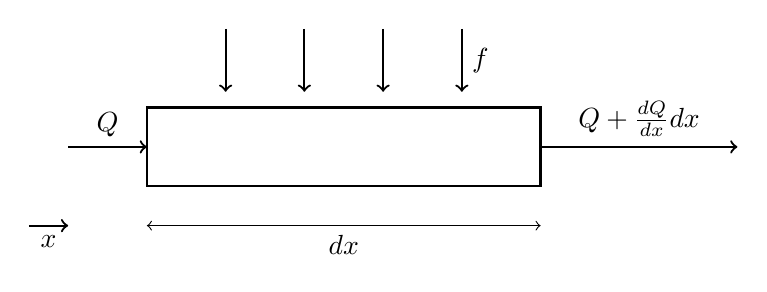
\begin{tikzpicture}
		
		% Draw the rectangle
		\draw[thick] (0,0) rectangle (5,1);
		
		% Arrows going into the rectangle with labels "f"
		\draw[->, thick] (1, 2) -- (1, 1.2);
		\draw[->, thick] (2, 2) -- (2, 1.2);
		\draw[->, thick] (3, 2) -- (3, 1.2);
		\draw[->, thick] (4, 2) -- (4, 1.2) node[midway, right] {$f$};
		
		% Label for dx
		\draw[<->] (0,-0.5) -- (5,-0.5) node[midway, below] {$dx$};
		
		% Label for Q on the left
		\draw[->, thick] (-1,0.5) -- (0,0.5) node[midway, above] {$Q$};
		
		% Label for Q+dQ/dx*dx on the right
		\draw[->, thick] (5,0.5) -- (7.5,0.5) node[midway, above] {$Q + \frac{dQ}{dx}dx$};
		
		% Arrow for x-axis direction
		\draw[->, thick] (-1.5,-0.5) -- (-1,-0.5) node[midway, below] {$x$};
		
	\end{tikzpicture}
	\end{center}
	
	\begin{equation}
		Q+fdx=Q+\frac{dQ}{dx}\cdot dx \Rightarrow f=\frac{dQ}{dx}
	\end{equation}
	
	\begin{equation}
		Q= -K_x \cdot \frac{dT}{dx} - \text{ закон Фурье}
	\end{equation}
	
	где $K_x=\lambda S$ - коэф. теплопроводности стержня, $\lambda$ - коэф. теплопроводности материала, 	$S$ - площадь сечения стержня.
	
	(2) $\rightarrow$ (1):
	\begin{equation}
	-\frac{d}{dx}(K_x \cdot \frac{dT}{dx}) = f
	\end{equation}
	
	\underline{Граничные условия:}
	\begin{enumerate}
		\item $T(0)=T_0, \ T(l)=T_l$
		\item $-K_x \cdot \dfrac{dT}{dx} |_{x=0} = q, \ -K_x \cdot \dfrac{dT}{dx} |_{x=l} = -q$
		\item $K_x \cdot  \dfrac{dT}{dx} |_{x=0} = -\alpha g (T_0 - T(0)), \ K_x \cdot \dfrac{dT}{dx} |_{x=l} = \alpha g (T_l - T(l))$
	\end{enumerate}
	
	\begin{center}
	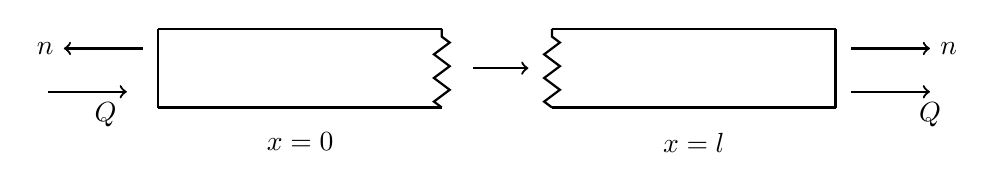
\begin{tikzpicture}
    % Левый конец стержня
    \draw[thick] (0.2,0) -- (3.8,0);
    \draw[thick] (0.2,1) -- (3.8,1);
    \draw[thick] (0.2,0) -- (0.2,1);
    \draw[thick, decorate, decoration={zigzag, segment length=3mm, amplitude=1mm}] (3.8,0) -- (3.8,1);

    % Правый конец стержня
    \draw[thick] (5.2,0) -- (8.8,0);
    \draw[thick] (5.2,1) -- (8.8,1);
    \draw[thick] (8.8,0) -- (8.8,1);
    \draw[thick, decorate, decoration={zigzag, segment length=3mm, amplitude=1mm}] (5.2,0) -- (5.2,1);
    
    % Силы
    \draw[->, thick] (0,0.75) -- (-1,0.75) node[left] { $n$};
    \draw[->, thick] (-1.2,0.2) -- (-0.2,0.2) node[below left] { $Q$};
    \draw[->, thick] (9,0.75) -- (10,0.75) node[right] { $n$};
    \draw[->, thick] (9,0.2) -- (10,0.2) node[below] { $Q$};

    % Обозначения координат
    \node[below] at (2,-0.2) { $x=0$};
    \node[below] at (7,-0.2) { $x=l$};
    
    \draw[->, thick] (4.2, 0.5) -- (4.9, 0.5);

\end{tikzpicture}
\end{center}
	
	Чтобы определить знак в граничных условиях второго рода нужно смотреть на направление $Q=K_x \cdot  \dfrac{dT}{dx}$.
	
	\underline{Интегральная формулировка:} $ \ r=-\dfrac{d}{dx}(K_x \cdot \dfrac{dT}{dx}) - f = 0, \quad v = \delta T $
	\begin{equation}
	\int\limits_0^l (-\frac{d}{dx}(K_x \cdot \frac{dT}{dx}) - f) \cdot \delta T \cdot S dx = 0 \Rightarrow \int\limits_0^l  \frac{d\delta T}{dx}(K_x \cdot \frac{dT}{dx}) \cdot S dx - F(\delta T) = 0
	\end{equation}
	\[
	 F(\delta T) = S(K_x \cdot \frac{dT}{dx})\cdot \delta T |_0^l = -SQ_l \cdot \delta T(l) + SQ_0 \cdot\delta T(0)
	 \]
	 \[  Q_0 = -K_x \cdot \frac{dT}{dx} |_{x=0}, Q_l = -K_x \cdot \frac{dT}{dx} |_{x=l}
	\]
	\[
	T= Nq = N_1^{(i)}T_i +  N_2^{(i)}T_{i+1}, \quad \frac{dT}{dx}=Bq
	\]
	\[ 	\delta T= N\delta q = N_1^{(i)}\delta T_i +  N_2^{(i)}\delta T_{i+1}, \quad \frac{d\delta T}{dx}=B\delta q
	\]
	
	\underline{Вариационная формулировка:}
	\[
		J(t) = \frac{1}{2} \int\limits_0^{l} K_x \left( \frac{dT}{dx} \right)^2 S \, dx - \int\limits_0^{l} SfT \ dx + S Q_l T_l - S Q_0 T_0 \rightarrow \min \quad \text{(совпадает с (4))} 
	\]
	\[
		\Delta J = J(T + \delta T) - J(T) = \frac{1}{2} \int\limits_0^{l} K_x S \left( \frac{d(T + \delta T)}{dx} \right)^2 dx - \int_0^{l} S f (T + \delta T) \, dx -
	\]
	\[  
		 \frac{1}{2} \int\limits_0^{l} K_x \left( \frac{dT}{dx} \right)^2 S \, dx +
		 \int\limits_0^{l} S f T \, dx + S Q_l (T_l + \delta T_l) - S Q_0 (T_0 -\delta T_0) -
		 S Q_l T_l + S Q_0 T_0 =
	\] 
	\[
		= \frac{1}{2} \int\limits_0^{l} S K_x \left[ \left( \frac{dT}{dx} \right)^2 + 2 \cdot \frac{dT}{dx} \cdot \frac{d \delta T}{dx} + \left( \frac{d \delta T}{dx} \right)^2 \right] dx - \int\limits_0^{l} S f \delta T \, dx -
	\]
	\[ \frac{1}{2} \int\limits_0^{l} S K_x \left( \frac{dT}{dx} \right)^2 dx + S Q_l \delta T_l - S Q_0 \delta T_0 
	\]
	
	Оставим линейную часть приращений $\Delta J$ относительно $\delta T$:
	\[
		\int\limits_0^{l} S K_x \frac{dT}{dx}\cdot \frac{d \delta T}{dx} \, dx - \int\limits_0^{l} S f \delta T \, dx + S Q_l \delta T_l - S Q_0 \delta T_0 \rightarrow (4)
	\]
   \newpage
   \section*{11/10}
	
		\begin{center}
		\textbf{Двумерные краевые задачи}
	\end{center}
	\begin{equation} \label{2d_eq}
	-\frac{\partial}{\partial x} \left( K \frac{\partial u}{\partial x} \right) -\frac{\partial}{\partial y} \left( K \frac{\partial u}{\partial y} \right) + bu = f
	\end{equation}
	
	$K(x, y),\ b(x, y),\ f(x,y)$ -- заданные (гладкие) функции.
	
	$u(x, y)$ -- неизвестная.
	
	$\Omega$ -- область, где задано уравнение \eqref{2d_eq}, $\Gamma$ -- граница $\Omega$ .
	\\
	
	\begin{center}
	\begin{tikzpicture}
    % Ось координат
    \draw[->] (-1,0) -- (5,0);
    \draw[->] (0,-1) -- (0,5);
    
    % Кардиоида
        \draw[domain=0:360,samples=200,smooth,variable=\t,rotate=-90,scale=0.5,shift={(3,3)}]
        plot ({2*(1-cos(\t)) * cos(\t) - 6}, {2*(1-cos(\t)) * sin(\t) + 2});
        
        \draw[->,color=red,domain=270:340,samples=200,smooth,variable=\t,rotate=-90,scale=0.5,shift={(3,3)}]
        plot ({2*(1-cos(\t)) * cos(\t) - 6}, {2*(1-cos(\t)) * sin(\t) + 2}) node[below] {$\xi$};
        
        \draw[thick,color=blue,domain=200:240,samples=200,smooth,variable=\t,rotate=-90,scale=0.5,shift={(3,3)}]
        plot ({2*(1-cos(\t)) * cos(\t) - 6}, {2*(1-cos(\t)) * sin(\t) + 2}) node[above left] {$\Gamma_1$};
        
        \draw[->] (3, 1.25) -- (3, 0.5) node[right] {$\vec n$};
        
        \node at (3, 2) {$\Omega$};
        \node at (4, 1.5) {$\Gamma_2$};
        
\end{tikzpicture}
\end{center}
	
	Замкнутый контур $\Gamma$ -- гладкий, за исключением конечного числа угловых точек, в которых внутренний угол $\alpha \in [0; \pi]$.
	\[\Gamma = \underbrace{\Gamma_1}_{\text{I рода}} \cup \underbrace{\Gamma_2}_{\text{II/III рода}}\]
	\begin{center}
		$u(\xi) = \hat u(\xi)$ -- на $\Gamma_1$ (заданное значение).
	\end{center}
	\[K(\xi)\frac{\partial u}{\partial n} = \hat \sigma (\xi) - \text{ на } \Gamma_2\]
	\[\frac{\partial u}{\partial n} = \frac{\partial u}{\partial x} l_x + \frac{\partial u}{\partial y} l_y,\ 
	\begin{cases}
	l_x = \cos(\alpha x) = \cos(\vec x, \vec n),\\
	l_y = \cos(\alpha y) = \cos(\vec y, \vec n),\\
	||\vec n|| = 1
	\end{cases}\]

\begin{center}
	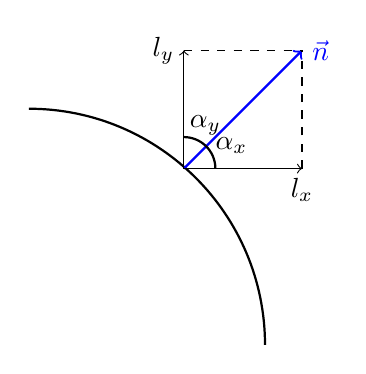
\begin{tikzpicture}
	\draw[thick] (0,0) arc[start angle=0, end angle=90, radius=3cm];

    	% Нормаль к гипотенузе
    	\coordinate (A) at (-0.18,0.93);
   	\coordinate (B) at (-2.5,2.93);
    	\coordinate (C) at (-2.5,0.93);
     	\coordinate (MidAB) at ($ (A)!0.5!(B) $);
	    
    	% Вектор нормали
    	\draw[->, thick, blue] (MidAB)++(0.31,0.31) -- ++(1.5,1.5) node[right] {$\vec n$};
	\draw[->] (MidAB)++(0.31,0.31) -- ++(0, 1.5) node[left] {$l_y$};
	\draw[->] (MidAB)++(0.31,0.31) -- ++(1.5, 0) node[below] {$l_x$};
	\draw[thick] (MidAB)++(0.71, 0.31) arc[start angle=0, end angle=47, radius=0.4cm] node[right] {$\alpha_x$};
	\draw[thick] (MidAB)++(0.31, 0.71) arc[start angle=90, end angle=47, radius=0.4cm] node[above] {$\alpha_y$};
	\draw[dashed] (MidAB)++(0.31,1.81) -- ++(1.5, 0);
	\draw[dashed] (MidAB)++(1.81,0.31) -- ++(0, 1.5);

	\end{tikzpicture}
	\end{center}
	
	Составим невязку:
	\[r(x, y) = -\frac{\partial}{\partial x} \left( K \frac{\partial u}{\partial x} \right) -\frac{\partial}{\partial y} \left( K \frac{\partial u}{\partial y} \right) + bu - f = 0\]
	
	\[\iint\limits_{\Omega} r(x, y) \cdot v \, dx \, dy = 0,\]
	
	где $v(x, y)$ -- пробная (гладкая) функция; на $\Gamma_1$: $v = 0$
	
	\begin{equation}\label{iint}
	\iint\limits_{\Omega} \left [ -\frac{\partial}{\partial x} \left( K \frac{\partial u}{\partial x} \right) -\frac{\partial}{\partial y} \left( K \frac{\partial u}{\partial y} \right) + bu - f \right ] \cdot v \, dx \, dy = 0
	\end{equation}
	
	Рассмотрим первый интеграл:
	\[-\iint\limits_{\Omega} \frac{\partial}{\partial x} \left( K \frac{\partial u}{\partial x} \right) \cdot v \, dx \, dy\]
	
	Формула Гаусса-Остроградского:
	\[\iint\limits_{\Omega} \frac{\partial}{\partial x} F dx dy = \int \limits_{\Gamma} F \cdot l_x d \xi\]
	
	Представим $F$ в виде $F = uv$:
	\[\frac{\partial}{\partial x} F = \frac{\partial}{\partial x} (uv) = \frac{\partial u}{\partial x} v + u \frac{\partial v}{\partial x}\ \Rightarrow\ 
	\frac{\partial u}{\partial x} v = \frac{\partial}{\partial x} (uv) - u \frac{\partial v}{\partial x}\]
	
	Отсюда:
	\[\iint\limits_{\Omega} \frac{\partial u}{\partial x} v \, dx \, dy = \iint\limits_{\Omega} \left( \frac{\partial}{\partial x} (uv) - u \frac{\partial v}{\partial x} \right) \, dx \, dy\]
	
	И по формуле Гаусса-Остроградского:
	\[\iint\limits_{\Omega} \frac{\partial u}{\partial x} v \, dx \, dy = \int \limits_{\Gamma} uv \cdot l_x d \xi - \iint\limits_{\Omega} \frac{\partial v}{\partial x} u \, dx \, dy\]
	
	Тогда:
	\[-\iint\limits_{\Omega} \frac{\partial}{\partial x} \left( K \frac{\partial u}{\partial x} \right) \cdot v \, dx \, dy = 
	-\int \limits_{\Gamma} K \cdot \frac{\partial u}{\partial x} \cdot v \cdot l_x d \xi + \iint\limits_{\Omega} \frac{\partial v}{\partial x} \left(  K \cdot \frac{\partial u}{\partial x} \right) \, dx \, dy\]
	\[-\iint\limits_{\Omega} \frac{\partial}{\partial y} \left( K \frac{\partial u}{\partial y} \right) \cdot v \, dx \, dy = 
	-\int \limits_{\Gamma} K \cdot \frac{\partial u}{\partial y} \cdot v \cdot l_y d \xi + \iint\limits_{\Omega} \frac{\partial v}{\partial y} \left(  K \cdot \frac{\partial u}{\partial y} \right) \, dx \, dy\]
	
	Подставим в \eqref{iint}:
	\[\iint\limits_{\Omega} \left [ \frac{\partial v}{\partial x} \cdot K \cdot \frac{\partial u}{\partial x} + \frac{\partial v}{\partial y} \cdot K \cdot \frac{\partial u}{\partial y} + bu \cdot v - f  \cdot v \right ] \, dx \, dy -\]
	\[-\int \limits_{\Gamma_2} K \cdot v \cdot \left(\frac{\partial u}{\partial x} \cdot l_x + \frac{\partial u}{\partial y} \cdot l_y \right) = 0\]

	\underline{Задача упругости}
 	$ u(x, y) $ - перемещения \\
 	\[ \varepsilon = [\varepsilon_x \quad \varepsilon_y]^T, \quad \varepsilon_x = - \frac{\partial u}{\partial y},\quad \varepsilon_y = - \frac{\partial u}{\partial y} \]
	\[ \varepsilon = Lu,\quad L = \left[- \frac{\partial}{\partial x} \quad - \frac{\partial}{\partial y}\right]^T \]
	\[ \sigma = k \varepsilon = kLu \]
	\begin{center}
	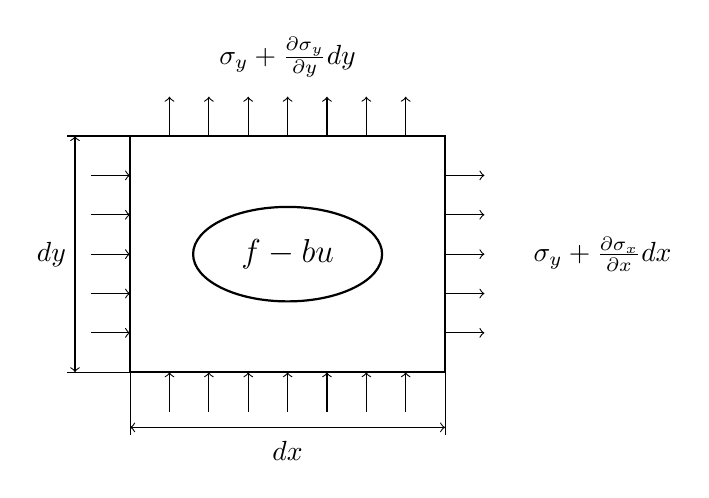
\begin{tikzpicture}
    % Прямоугольник
    \draw[thick] (0, 0) rectangle (4, 3);
    
    % Центральная фигура (овал)
    \draw[thick] (2, 1.5) ellipse (1.2 and 0.6);
    \node at (2, 1.5) {\large $f - bu$};  % Текст внутри овала
    
    % Горизонтальные стрелки (слева направо)
    \foreach \y in {0.5, 1, 1.5, 2, 2.5} {
        \draw[->] (-0.5, \y) -- (0, \y);
    }
    
    % Вертикальные стрелки (снизу вверх)
    \foreach \x in {0.5, 1, 1.5, 2, 2.5, 3, 3.5} {
        \draw[->] (\x, -0.5) -- (\x, 0);
    }

    % Горизонтальные стрелки справа
    \foreach \y in {0.5, 1, 1.5, 2, 2.5} {
        \draw[->] (4, \y) -- (4.5, \y);
    }
    
    % Вертикальные стрелки сверху
    \foreach \x in {0.5, 1, 1.5, 2, 2.5, 3, 3.5} {
        \draw[->] (\x, 3) -- (\x, 3.5);
    }
    
    % Подписи координат
    \draw[thin] (0, 0) -- (0, -0.8);
    \draw[thin] (4, 0) -- (4, -0.8);
    \draw[<->][thin] (0, -0.7) -- (4, -0.7);
    \node at (2, -1) {$dx$};    % Горизонтальная разметка снизу
    
    \draw[thin] (0, 0) -- (-0.8, 0);
    \draw[thin] (0, 3) -- (-0.8, 3);
    \draw[<->][thin] (-0.7, 0) -- (-0.7, 3);
    \node at (-1, 1.5) {$dy$};  % Вертикальная разметка слева
    
    \node at (2, 4) {$\sigma_y + \frac{\partial \sigma_y}{\partial y} dy$};
    \node at (6, 1.5) {$\sigma_y + \frac{\partial \sigma_x}{\partial x} dx$};

    % Дополнительные стрелки от центрального овала
    %\foreach \angle in {-40, -20, 0, 20, 40} {
        %\draw[->] (2, 1.5) -- ++(\angle:1.5);
   % }

\end{tikzpicture}
\end{center}
	\[ d \Omega = dxdy \]
	\[ \sigma_x dy + \sigma_y dx + (f-bu) dxdy = \left(\sigma_x + \frac{\partial \sigma_x}{\partial x}dx\right) dy + \left(\sigma_y + \frac{\partial \sigma_y}{\partial y}dy\right) dx \]
	\[ \frac{\partial \sigma_x}{\partial x} + \frac{\partial \sigma_y}{\partial y} = f - bu \]
	\[ L_* = \left[\frac{\partial}{\partial x} \quad \frac{\partial}{\partial y}\right],\quad L_* = -L^T,\ \  L_* \sigma = L_*kLu = f - bu \]
	\[ \left[\frac{\partial}{\partial x} \quad \frac{\partial}{\partial y}\right] \cdot k \cdot 
	\begin{bmatrix}
		-\frac{\partial u}{\partial x}\\
		- \frac{\partial u}{\partial y}
	\end{bmatrix}
 	= f-bu \]
	\[-\frac{\partial}{\partial x} \left ( K \frac{\partial u}{\partial x} \right) - \frac{\partial}{\partial y} \left ( K \frac{\partial u}{\partial y} \right) = f \cdot bu \Leftrightarrow \eqref{2d_eq}\]
	
	\begin{center}
	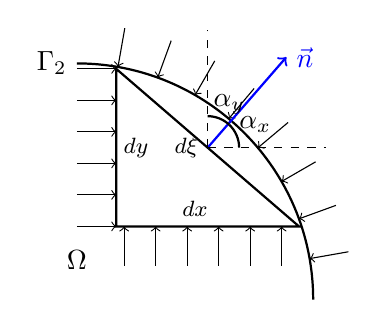
\begin{tikzpicture}
	\draw[thick] (0,0) arc[start angle=0, end angle=90, radius=3cm] node[left] {$\Gamma_2$};
	\foreach \angle in {10, 20, 30, 40, 50, 60, 70, 80} {
        % Координаты точек на окружности
        \coordinate (P) at ({3*cos(\angle) - 3}, {3*sin(\angle)});
        % Координаты направления нормали
        \coordinate (N) at ({0.5*cos(\angle)}, {0.5*sin(\angle)});
        % Рисуем нормали
        \draw[<-] (P) -- ++(N);
    }

	\draw[thick] (-0.18,0.93) -- (-2.5,2.93) -- (-2.5,0.93) -- cycle;
	\node at (-1.5, 1.15) {\footnotesize$dx$};
	\node at (-2.25, 1.93) {\footnotesize$dy$};

    	% Нормаль к гипотенузе
    	\coordinate (A) at (-0.18,0.93);
   	\coordinate (B) at (-2.5,2.93);
    	\coordinate (C) at (-2.5,0.93);
     	\coordinate (MidAB) at ($ (A)!0.5!(B) $);
	
	\node[left] at (MidAB) {\footnotesize$d\xi$};
    
    	% Вектор нормали
    	\draw[->, thick, blue] (MidAB) -- ++(1,1.15) node[right] {$\vec n$};
	\draw[dashed] (MidAB) -- ++(0, 1.5);
	\draw[dashed] (MidAB) -- ++(1.5, 0);
	\draw[thick] (MidAB)++(0.4, 0) arc[start angle=0, end angle=47, radius=0.4cm] node[right] {$\alpha_x$};
	\draw[thick] (MidAB)++(0, 0.4) arc[start angle=90, end angle=47, radius=0.4cm] node[above] {$\alpha_y$};
	
	\draw[->] (-3,0.93) -- (-2.5,0.93);
	\draw[->] (-3,1.33) -- (-2.5,1.33);
	\draw[->] (-3,1.73) -- (-2.5,1.73);
	\draw[->] (-3,2.13) -- (-2.5,2.13);
	\draw[->] (-3,2.53) -- (-2.5,2.53);
	\draw[->] (-3,2.93) -- (-2.5,2.93);
	
	\draw[->] (-2.4,0.43) -- (-2.4,0.93);
	\draw[->] (-2,0.43) -- (-2,0.93);
	\draw[->] (-1.6,0.43) -- (-1.6,0.93);
	\draw[->] (-1.2,0.43) -- (-1.2,0.93);
	\draw[->] (-0.8,0.43) -- (-0.8,0.93);
	\draw[->] (-0.4,0.43) -- (-0.4,0.93);
	
	\node at (-3, 0.5) {$\Omega$};
	\end{tikzpicture}
	\end{center}
	\[\Gamma_1: u(\xi) = \hat u(\xi)\]
	\[dx = \cos \alpha_y d\xi = l_y d\xi,\ \ dy = \cos \alpha_x d\xi = l_x d\xi\]
	\[\sigma_y dx + \sigma_x dy + \hat \sigma d\xi = 0,\ \ \sigma_x = K \varepsilon_x = -K \frac{\partial u}{\partial x},\ \sigma_y = K \varepsilon_y = -K \frac{\partial u}{\partial y}\]
	
	Тогда:
	\[-K \frac{\partial u}{\partial y} dx -K \frac{\partial u}{\partial x} dy + \hat \sigma d\xi = 0,\ \ -K \frac{\partial u}{\partial y} l_y d\xi -K \frac{\partial u}{\partial x} l_x d\xi + \hat \sigma d\xi = 0\]
	\[K \frac{\partial u}{\partial n} = \hat \sigma\]
	
	Отсюда:
	\begin{equation}\label{2d_eq_2}
	\iint \limits_{\Omega} \left(\frac{\partial v}{\partial x} K \frac{\partial u}{\partial x} + \frac{\partial v}{\partial y} K \frac{\partial u}{\partial y} + bu \cdot v - f \cdot v\right) dx dy - \\
	\int \limits_{\Gamma} \underbrace{ \left(K \frac{\partial u}{\partial x} l_x + K \frac{\partial u}{\partial y} l_y\right)}_{K \cdot \frac{\partial u}{\partial n} = \hat \sigma(\xi)}  \cdot v d\xi = 0 
	\end{equation}
	
	\[\iint \limits_{\Omega} ((Lu)^T K (Lu) + v^T bu - v^T f) dxdy - \int \limits_{\Gamma_2} v^T \hat \sigma d\xi = 0\]
   \newpage

   \end{document}
   